
\documentclass[xcolor=x11names,compress,10pt,handout]{beamer}

%% Beamer Layout %%%%%%%%%%%%%%%%%%%%%%%%%%%%%%%%%%
\useoutertheme[subsection=false,shadow]{miniframes}
\useinnertheme{default}
\usefonttheme{serif}
%\usepackage{palatino}
\usepackage{xcolor}

\usepackage{listings}
\usepackage{courier}
\lstset{basicstyle=\footnotesize\ttfamily,breaklines=true}
\lstset{
  backgroundcolor=\color{gray!5}, %\color{white!95!blue},
  basicstyle=\footnotesize\tt,     % the size of the fonts that are used for the code
  breakatwhitespace=false,         % sets if automatic breaks should only happen at whitespace
  breaklines=true,                 % sets automatic line breaking
  captionpos=b,                    % sets the caption-position to bottom
  rulecolor=\color{gray},
  extendedchars=true,              % lets you use non-ASCII characters; for 8-bits encodings only, does not work with UTF-8
  frame=single,                    % adds a frame around the code
  keywordstyle=\bf,
  showspaces=false,                % show spaces everywhere adding particular underscores; it overrides 'showstringspaces'
  showstringspaces=false,          % underline spaces within strings only
  showtabs=false,                  % show tabs within strings adding particular underscores
  tabsize=2                        % sets default tabsize to 2 spaces
}

\definecolor{bblue}{RGB}{13,64,130}

\newenvironment{changemargin}[2]{% 
  \begin{list}{}{% 
    \setlength{\topsep}{0pt}% 
    \setlength{\leftmargin}{#1}% 
    \setlength{\rightmargin}{#2}% 
    \setlength{\listparindent}{\parindent}% 
    \setlength{\itemindent}{\parindent}% 
    \setlength{\parsep}{\parskip}% 
  }% 
  \item[]}{\end{list}}

\setbeamercolor*{lower separation line head}{bg=bblue} 
\setbeamercolor*{normal text}{fg=black,bg=white} 
\setbeamercolor*{alerted text}{fg=red} 
\setbeamercolor*{example text}{fg=black} 
\setbeamercolor*{structure}{fg=bblue} 
 
\setbeamercolor*{palette tertiary}{fg=black,bg=black!10} 
\setbeamercolor*{palette quaternary}{fg=black,bg=black!10} 

\renewcommand{\(}{\begin{columns}}
\renewcommand{\)}{\end{columns}}
\newcommand{\<}[1]{\begin{column}{#1}}
\renewcommand{\>}{\end{column}}


\newenvironment<>{block1}[1]{%
  \setbeamercolor{block title}{fg=black,bg=bblue!15!white}%
  \begin{block}#2{#1}}{\end{block}}
  
  
\newenvironment<>{block2}[1]{%
  \setbeamercolor{block title}{fg=white,bg=bblue!75!black}%
  \begin{block}#2{#1}}{\end{block}}

\newcommand{\by}{\mathbf{y}}
\newcommand{\bphi}{\boldsymbol{\phi}}

\setbeamercolor{block body}{fg=black,bg=gray!7}

\usepackage[absolute,overlay]{textpos}

% LOGO
\newcommand\FrameText[1]{%
  \begin{textblock*}{0.8\paperwidth}(40pt,.82\textheight)
    \raggedright #1\hspace{.5em}
  \end{textblock*}}
  
%\setbeamerfont{title like}{shape=\scshape}
\setbeamerfont{frametitle}{shape=\bf} 

\begin{document}


%%%%%%%%%%%%%%%%%%%%%%%%%%%%%%%%%%%%%%%%%%%%%%%%%%%%%%
%%%%%%%%%%%%%%%%%%%%%%%%%%%%%%%%%%%%%%%%%%%%%%%%%%%%%%
\begin{frame}
\title[]{\Large\bf
         
\includegraphics[scale=.25]{Bergm_logo.pdf}\\[-.3cm] 
         \textcolor{black}{Brief Intro - Basic functions}}
%\subtitle[]{(Chapter 6 of the manual)}
  
\author[]{{\large Alberto Caimo}\\ 
          \textcolor{blue}{\bfseries\ttfamily acaimo.github.io}
          }

\institute[]
  {\normalsize }

\date[]
  {}

\titlepage
 
 %\FrameText{ \centering
 %
\includegraphics[width=.8\textwidth]{ssnar_logo_slides}}

\end{frame}


%%
%\begin{frame}{Outline}
%\tableofcontents
%\end{frame}

%%
% \begin{itemize}
% \item
% \end{itemize}


%
\begin{frame}[fragile]{} 
\begin{block1}{\bf Definitions and notation}
\begin{itemize}
\item Networks are generally represented by graphs of nodes (actors) and edges (relations)
\item $N$ number of nodes ({\bf fixed})
\item $Y$ {\bf random} $N \times N$ adjacency matrix where: 
 \begin{itemize} 
 \item $Y_{ij} = 1$, if $i$ and $j$ are connected
 \item $Y_{ij} = 0$, if $i$ and $j$ are not connected
 \end{itemize}
\item $y$ realisation of $Y$
\end{itemize}
\end{block1}  
\begin{changemargin}{-.7cm}{0cm}
\begin{figure}[htp]
  \centering
  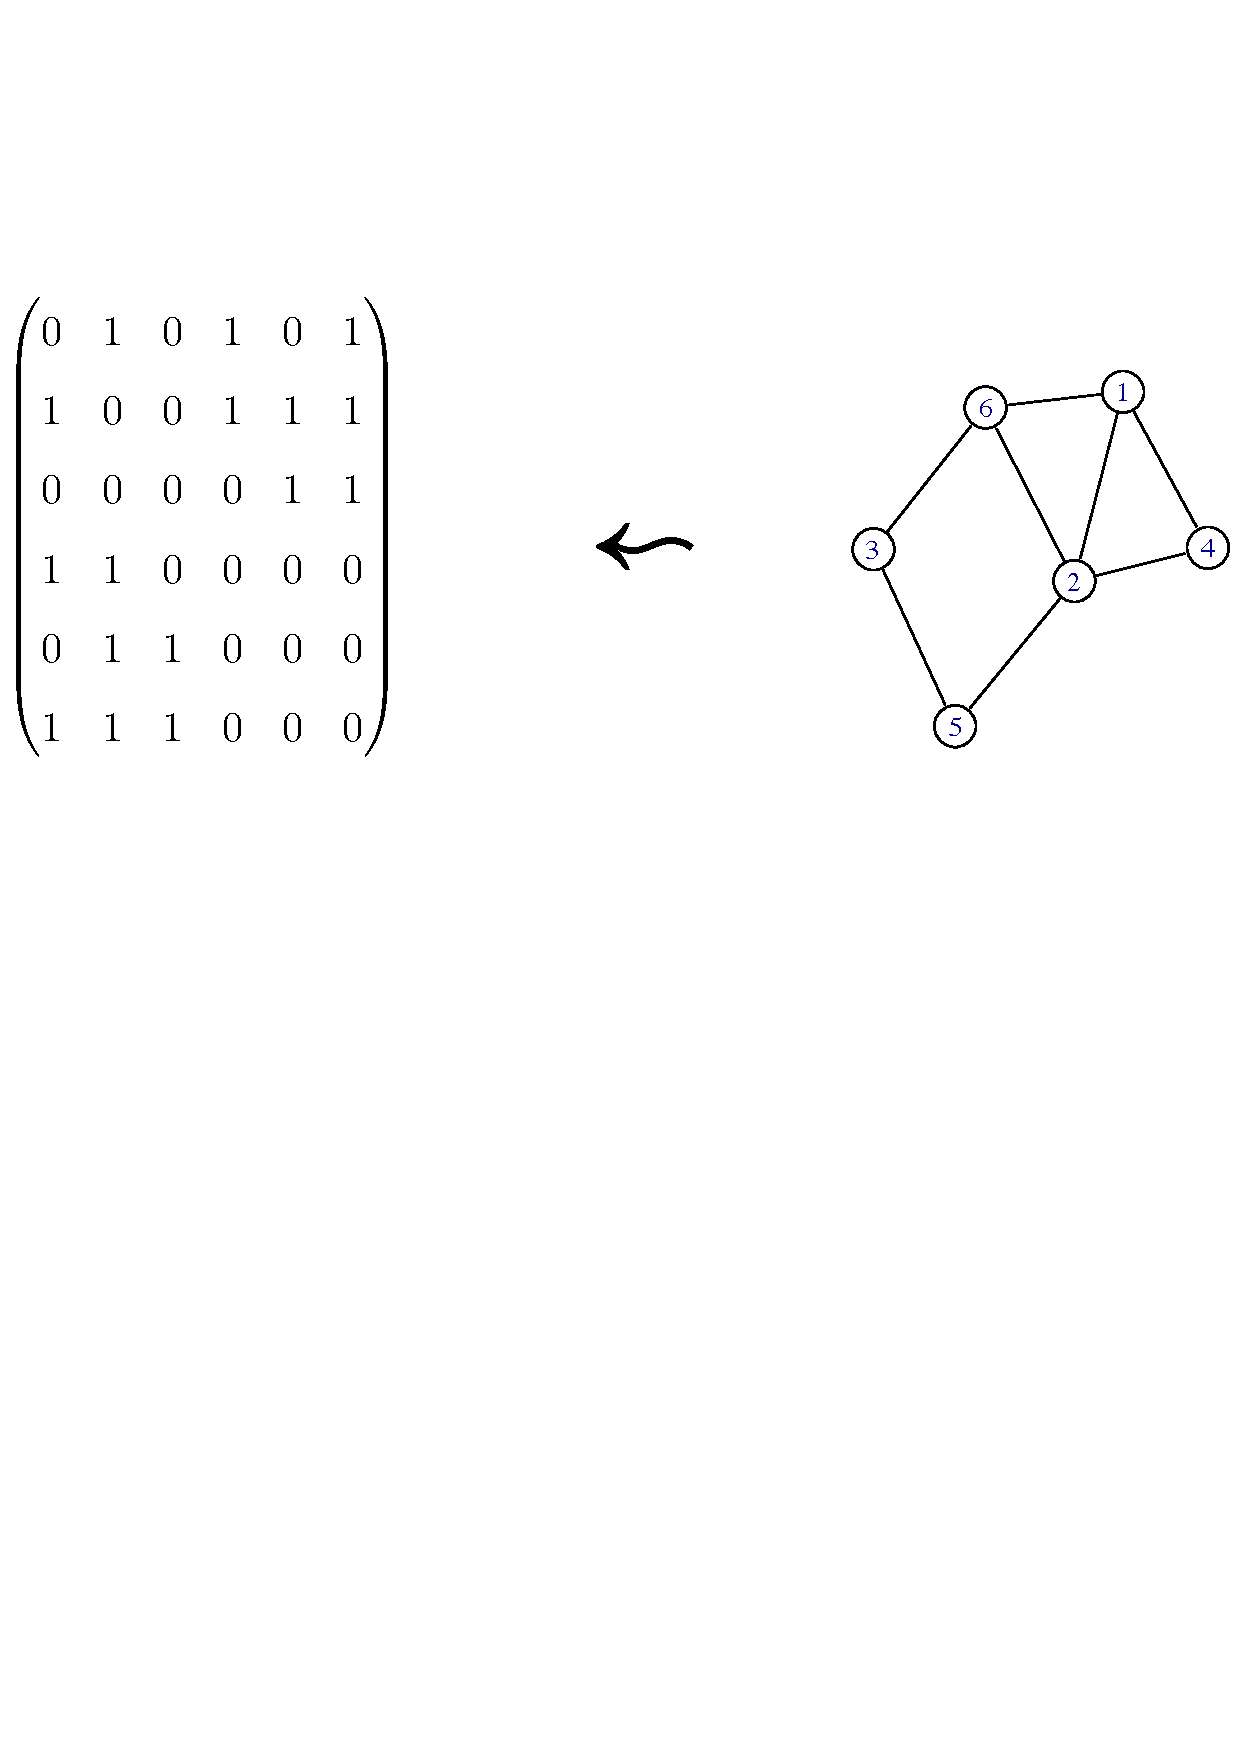
\includegraphics[scale=.4]{Y.pdf}
\end{figure}
\end{changemargin} 
\end{frame}

%
\begin{frame}[fragile]{Exponential random graph models (ERGMs)} 

\begin{block1}{\bf Basic assumptions}
\begin{itemize}
\item The observed network $y$ is generated by a stochastic process in which edges are created because of the presence or absence of other edges.
\item Local effects are represented by {\bf network statistics} $s(y)$ that generate dyadic relations and may depend on the surrounding environment.\\[.3cm]
\end{itemize} 
\end{block1}

For example:
\begin{itemize}
\item Similar attributes are generally more likely to form friendship edges ({\bf homophily})
\item Two nodes connected to a third node are likely to form an edge between them ({\bf clustering})
\end{itemize}
\end{frame}

%
\begin{frame}[fragile]{Exponential random graph models (ERGMs)} 
\begin{block1}{\bf Definition}
$$
\Pr(Y = y) = \frac{\exp\{\theta^T s(y)\}}{c(\theta)}
$$
\end{block1}

\begin{itemize}
\item Describe the probability of $y$ as a function of the parameter $\theta$;
\item $s(y)$ is a vector of network statistics (e.g. number of edges, number of triangles, etc.) associated to effects of interest;
\item $\theta$ is the vector of parameters associated to the network statistics $s(y)$;
\item $c(\theta)$ is a normalising constant which is \textcolor{red}{\bf intractable} for not trivially small networks.
\end{itemize}
\end{frame}

%%
%\begin{frame}[fragile]{Dependence assumptions and network statistics} 
%\begin{itemize}
%\item Dyadic dependence (as in the random graph model) is an unrealistic assumption in many circumstances;
%\item Network statistics involving more than a dyad imply {\bf dependence} between dyads: an edge between node $i$ and $j$ is assumed to be dependent on the presence of other edges.\\[.3cm]
%\end{itemize}
%
%For example:
%\begin{itemize}
%\item {\bf Stars} statistics assume that an edge between $i$ and $j$ is contingent on any possible edge involving node $i$ and $j$ (i.e. on the degrees of $i$ and $j$).
%\item {\bf Triadic} statistics assume that an edge between $i$ and $j$ is contingent on any possible edge involving any node of the network connected to both $i$ and $j$.
%\end{itemize}
%\end{frame}




%
\begin{frame}[fragile]{Bayesian inference for ERGMs with {\sf Bergm}}  
Bayesian inference for ERGMs is based on the posterior distribution of $\theta$ given the data $y$:
$$
p(\theta | y)  
= \frac{ \exp \{ \theta^t s(y)\} }
       {c(\theta)}\; \frac{p(\theta)}{p(y)},
$$
where:
\begin{itemize}
\item $p(\theta)$ is the prior distribution of the parameter 
\item $p(y)$ is the marginal likelihood of $y$ which is typically \textcolor{red}{\bf intractable}.
\end{itemize}
\end{frame}

% 
\begin{frame}[fragile]{Bayesian inference for ERGMs with {\sf Bergm}} 
\begin{itemize} 
 \item \textcolor{blue}{\sf Bergm} is an {\sf R} package which provides a comprehensive framework for Bayesian estimation and model adequacy for ERGMs using advanced Monte Carlo algorithms (see, e.g., Caimo and Friel, 2011).
\item \textcolor{blue}{\sf Bergm} is based on the \textcolor{blue}{\sf statnet} suite of packages (Handcock et al., 2007) and makes use of the same model set-up and network simulation procedures.
\end{itemize}
\end{frame}

%
\begin{frame}[fragile]{The {\sf Bergm} package}  
\begin{block1}{\bf Main functions}
\begin{itemize}
\item $\textcolor{blue}{\mathtt{bergm()}}$: function to fit Bayesian exponential random graphs models using the approximate exchange algorithm
\item $\textcolor{blue}{\mathtt{bergm.output()}}$: function to return the posterior parameter density estimate and creates simple diagnostic plots for the MCMC produced from a fit.
\item $\textcolor{blue}{\mathtt{bgof()}}$: function to calculate summaries for degree, minimum geodesic distances, and edgewise shared partner distributions to diagnose Bayesian goodness-of-fit.
\end{itemize} 
\end{block1}
\end{frame}

%
\begin{frame}[fragile]{Example - {\sf Bergm} in action!} 
\lstset{
    escapeinside={(*}{*)}
}
\begin{lstlisting}
library(statnet)
data(zach) (*\textcolor{red}{\# 34 interacting members of a karate club}*)
y <- zach
plot(y, vertex.col = "skyblue", vertex.cex = 2)
\end{lstlisting}  
\begin{figure}[htp]
  \centering
  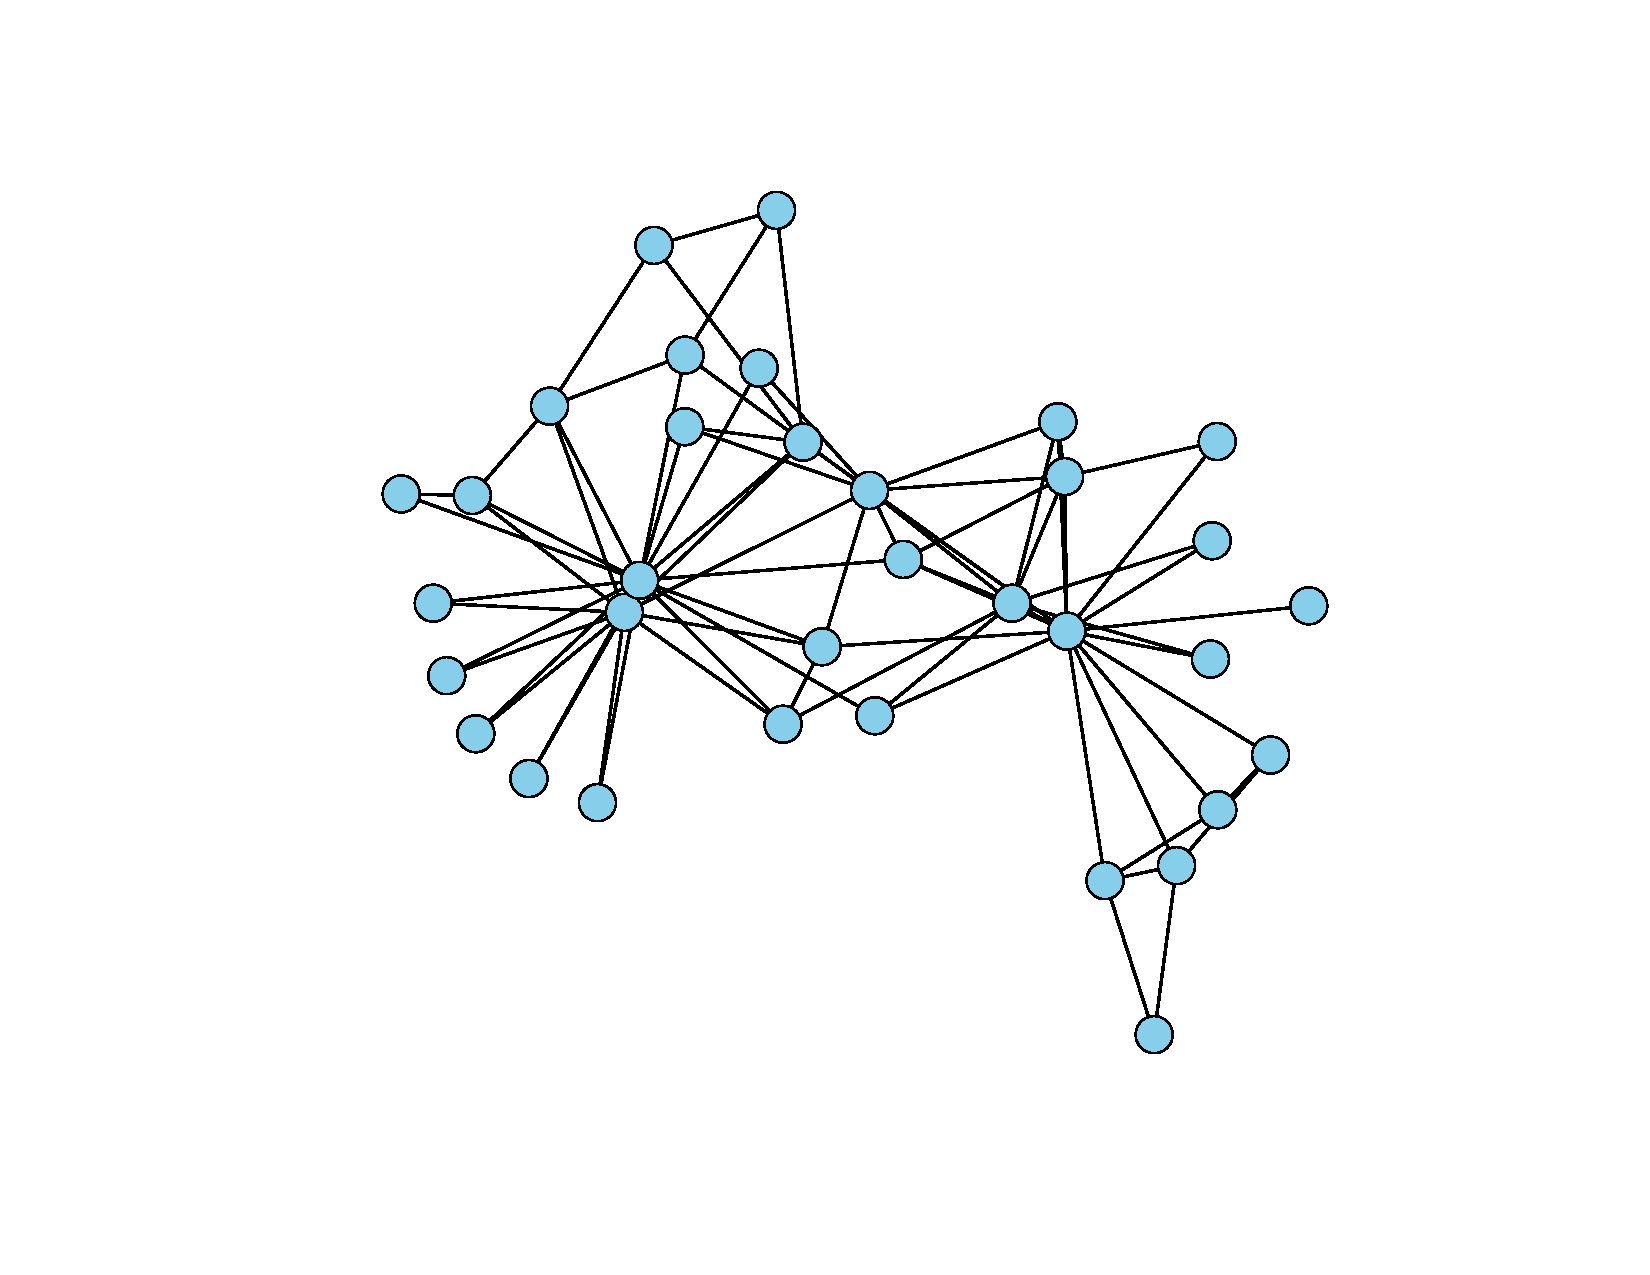
\includegraphics[scale=.35]{zach_graph.pdf}
\end{figure}     
\end{frame}

%
\begin{frame}[fragile]{Example - {\sf Bergm} in action!}

{\bf ERGM specification}: 
$$
\Pr(Y = y) \propto \exp \{ \theta_1\ \mathrm{edges}(y) + \theta_2\ \mathrm{gwdegree}(y) + \theta_3\ \mathrm{gwesp}(y) \} 
$$
\begin{changemargin}{-.7cm}{0cm}
\begin{figure}[htp]
  \centering
  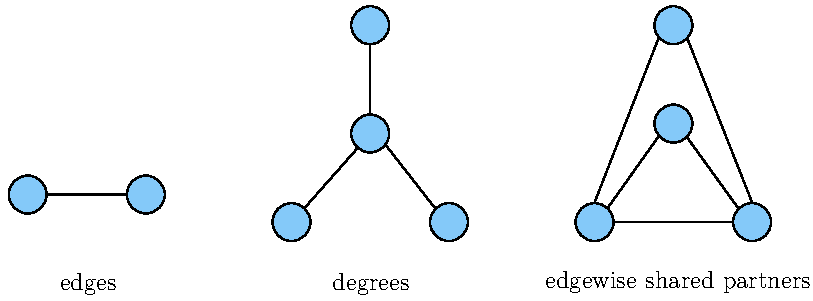
\includegraphics[scale=.7]{stats.pdf}
\end{figure}
\end{changemargin} 
\begin{lstlisting}
library(Bergm)

model <- y ~ edges +
             gwdegree(0.2, fixed = TRUE) +
             gwesp(0.2, fixed = TRUE)
\end{lstlisting}
\end{frame}

%
\begin{frame}[fragile]{Example - {\sf Bergm} in action!}

{\bf Prior specification}:
\begin{itemize}
\item vague normal prior distribution with no correlation between the parameters; 
\item we assume low density of the network: $\theta_1 < 0$;\\[.4cm]  
\end{itemize}
So, for example:
$$
\theta \sim N \left(\begin{bmatrix}
-2\\ 
0\\ 
0
\end{bmatrix},
\begin{bmatrix}
5 & 0 & 0  \\ 
0 & 5 & 0  \\  
0 & 0 & 5  \\ 
\end{bmatrix}
\right)
$$ 
\begin{lstlisting}
mean.prior <- c(-2, 0, 0)
sigma.prior <- diag(5, 3)
\end{lstlisting}
\end{frame}



%
\begin{frame}[fragile]{Example - {\sf Bergm} in action!} 

The {\bf approximate exchange algorithm} ($\textcolor{blue}{\mathtt{bergm()}}$ function):\\[.3cm]

\hrule\ \\[.2cm]
for $\textcolor{blue}{\mathtt{main.iters} \times \mathtt{n.chains}}$ iterations:\\
\vspace{.2cm}
\qquad 1. simulate $\theta'$ from $\epsilon(\cdot|\theta, \textcolor{blue}{\mathtt{gamma}})$\\
\vspace{.2cm}
\qquad 2. simulate $y'$ from $f(\cdot|\theta')$ using $\textcolor{blue}{\mathtt{aux.iters}}$ iterations\\
\vspace{.2cm}
\qquad 3. update $\theta \rightarrow \theta'$ with the log of the probability:
\begin{equation*}
\min\left( 0,\; \left[ \theta - \theta'\right]^t \left[s(y') - s(y)\right]
  +\log
   \frac{p(\theta')}
        {p(\theta)}\right)
\end{equation*}
\vspace{.2cm}
end for
\hrule
\end{frame}

%
\begin{frame}[fragile]{Example - {\sf Bergm} in action!}

\lstset{
    escapeinside={(*}{*)}
}
\begin{lstlisting}
posterior <- bergm(
    model,
    main.iters = 1500,
    n.chains = 6, (*\textcolor{red}{\# 6$\times$1.5k = 9k iterations}*)
    aux.iters = 3000, (*\textcolor{red}{\# for network simulation}*)
    (*\bfseries gamma = 0.9*), (*\textcolor{red}{\# tuned to get $\sim$20\% acceptance rate}*)
    mean.prior = mean.prior,
    sigma.prior = sigma.prior) 
        
bergm.output(posterior)
\end{lstlisting}
\lstset{basicstyle = \ttfamily\scriptsize, backgroundcolor=\color{white}}
\begin{lstlisting}
## Posterior Density Estimate for Model: 
## y ~ edges + gwdegree(0.2, fixed = TRUE) + gwesp(0.2, fixed = TRUE) 
##  
##                         Mean        SD    Naive SE Time-series SE
## theta1 (edges)     -3.810812 0.3650827 0.003848309     0.01942382
## theta2 (gwdegree)   5.169665 3.0124907 0.031754440     0.16939821
## theta3 (gwesp)      1.347093 0.2483486 0.002617824     0.01265695
## 
##                         2.5%       25%       50%       75%     97.5%
## theta1 (edges)     -4.501821 -4.053643 -3.811498 -3.565977 -3.107281
## theta2 (gwdegree)   0.913240  2.875273  4.633890  7.005652 12.135357
## theta3 (gwesp)      0.874649  1.178549  1.353660  1.514104  1.830226
## 
## Acceptance rate: 0.201 
\end{lstlisting}
\end{frame}

%
\begin{frame}[fragile]{Example - {\sf Bergm} in action!}
\begin{figure}[htp]
  \centering
  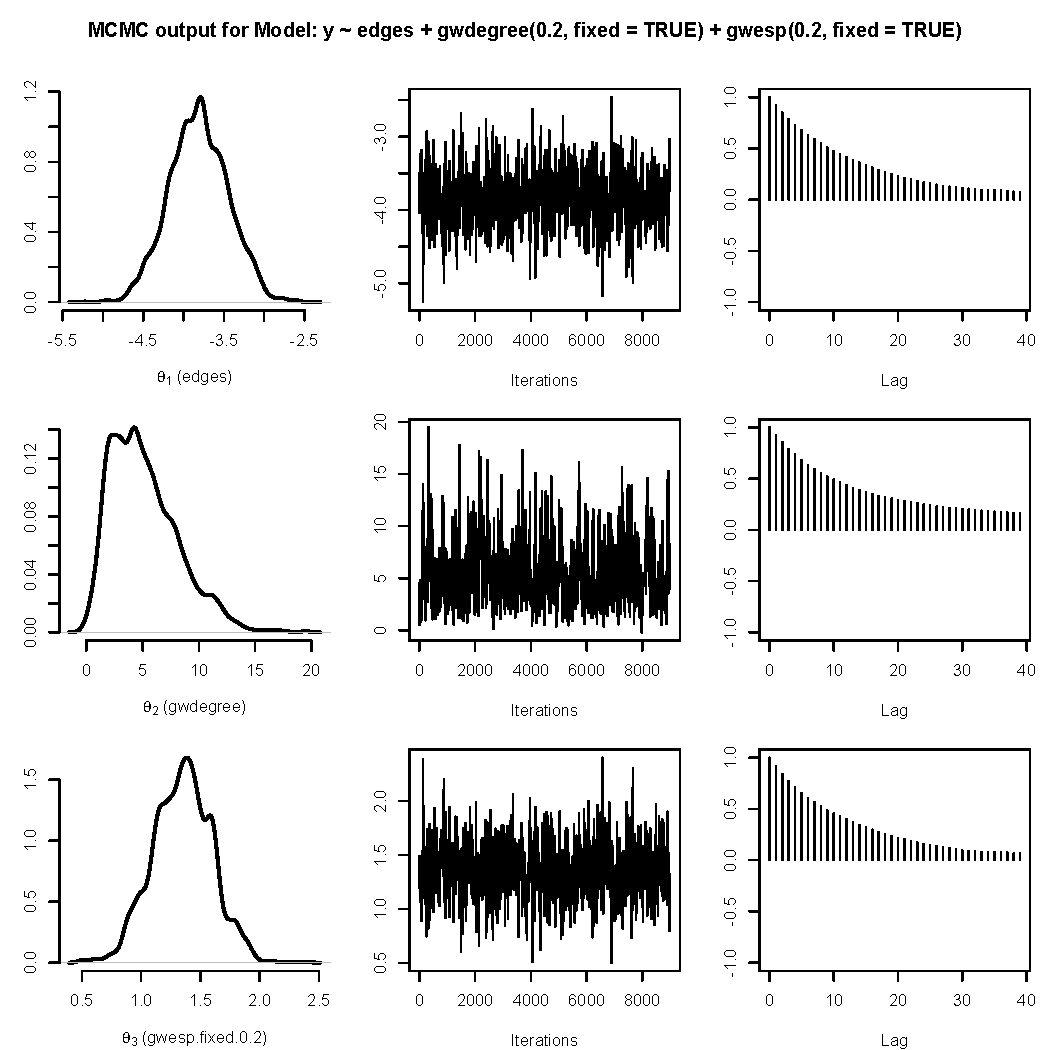
\includegraphics[scale=.45]{traces.pdf}
\end{figure}
\end{frame}


%
\begin{frame}[fragile]{Example - {\sf Bergm} in action!}

{\bf Bayesian GoF diagnostics} ($\textcolor{blue}{\mathtt{bgof()}}$ function):\\[.2cm]
\begin{itemize}
\item[1.] Draws $\textcolor{blue}{\mathtt{sample.size}}$ parameters $\{\tilde{\theta}_1, \tilde{\theta}_2, \cdots\}$ from the estimated posterior\\[.2cm]
\item[2.] Simulate networks $\{\tilde{y}_1, \tilde{y}_2, \cdots\}$ from each $\{\tilde{\theta}_1, \tilde{\theta}_2,\cdots\}$ using $\textcolor{blue}{\mathtt{aux.iters}}$ iterations\\[.2cm]
\item[3.] Compare some network statistics distributions of the $\{\tilde{y}_1, \tilde{y}_2, \cdots\}$ to the observed network $y$
\end{itemize}
\end{frame}

%
\begin{frame}[fragile]{Example - {\sf Bergm} in action!}
\begin{lstlisting}
bgof(posterior, sample.size = 100, aux.iters = 3000, 
     n.deg = 18, n.dist = 10, n.esp = 8)
\end{lstlisting}
\begin{changemargin}{-.7cm}{0cm}
\begin{figure}[htp]
  \centering
  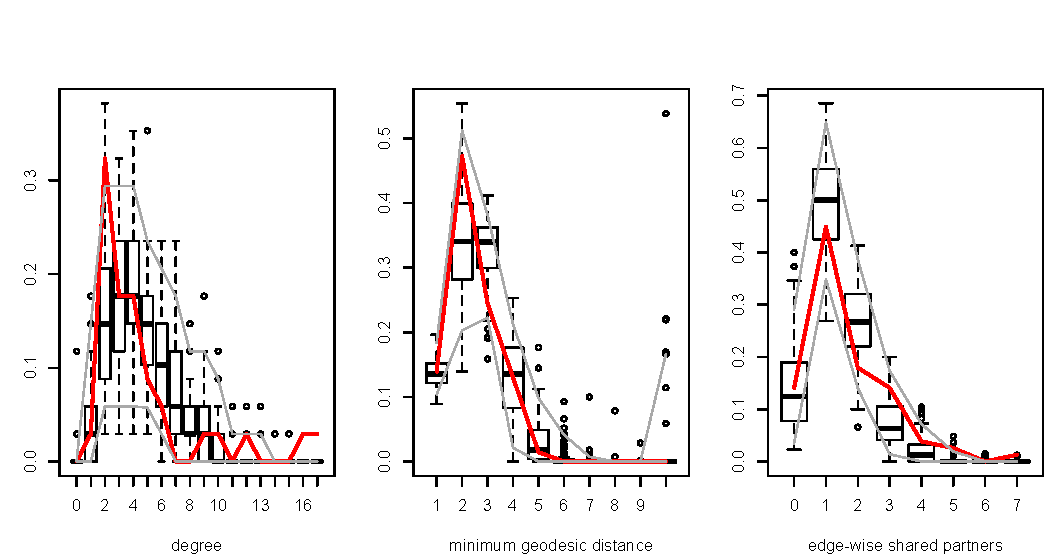
\includegraphics[scale=.68]{bgof.pdf}
\end{figure}
\end{changemargin}
\end{frame}



\end{document}














